% Úvod
%---------------------------------------------------------------------------
\chapter{Úvod}
Tradičné redakčné systémy pre správu obsahu sú obvykle zostavené z~dvoch hlavných súčastí -- \emph{administračného} a \emph{verejného webového rozhrania}. Administračné rozhranie slúži pre tvorbu a úpravu obsahu, webové na jeho nasledné zobrazenie. Webové rozhranie je typicky jednotné pre všetky typy zariadení na ktorých je zobrazované, tzn. že jeho používanie často nie je optimálne (napr. na mobilných telefónoch s dotykovou obrazovkou).

Pre tento dôvod sa začali využívať systémy bez webového rozhrania, disponujúce klasickým administračným a \emph{otvoreným aplikačným rozhraním} (API\footnote{API -- Application programming interface}), ktoré umožňuje obsah získať a následne ho zobraziť optimálne na ľubovoľnej platforme. Takéto redakčné systémy sa nazývajú \emph{Headless CMS}. Súčasné Headless CMS sú často robustné systémy, ktoré však vyžadujú komplexnú konfiguráciu predtým, ako ich je možné začať využívať. Niektoré takéto systémy potrebujú aj vlastnú infraštruktúru pre ich nasadenie. Tieto skutočnosti otvárajú priestor pre taký Headless CMS, ktorý by pomohol vyriešiť tieto prekážky. Takýto redakčný systém je cieľom tejto práce.

Navrhovaný systém poskytuje možnosť správy obsahu bez nutnosti úvodnej konfigurácie a infraštruktúry. Obsah je možné spravovať pomocou užívateľského rozhrania v~aplikácii Slack alebo doplnkového webového rozhrania.

\subsection*{Obsah kapitol}
% TODO: Add introduction to document's structure.

% Vývoj klientských aplikácii
%---------------------------------------------------------------------------
\chapter{Vývoj klientských aplikácii}
\label{theory:client_dev}
Zobrazenie obsahu užívateľom. Kapitola popisuje teoretické znalosti nutné pre návrh a implementáciu klientských aplikácií (v~prípade tejto práce webovej stránky a Slack aplikácie). Webové technológie sa vyvíjajú vysokou rýchlosťou a s~nimi aj nároky užívateľov na rýchlosť, použiteľnosť, ale aj vzhľad takýchto aplikácií.

Sekcia \ref{theory:UX} sa venuje základným pravidlám user experience\footnote{user experience -- uživateľská skúsenosť}, sekcie \ref{theory:HTML} až \ref{theory:typescript} približujú programovacie a značkovacie jazyky, ktoré sú použité v tejto práci. Posledné sekcie \ref{theory:react} a \ref{theory:nextjs} popisujú dve hlavné knižnice využívané pre vývoj moderných webových aplikácií React a Next.js.

% User Experience (UX)
\section{User experience (UX)}
\label{theory:UX}
Prí návrhu uživateľského rozhrania je jedným z~najdôležiteľších parametrov \emph{uživateľská skúsenosť}. Dizajnéri sa snažia zaistiť aby ich návrh bol intuitívny, jednoduchý, ale zároveň aj plne použiteľný a originálny. Pri UX analýze sa dizajnér snaží vnímať svoj návrh zo strany koncového užívateľa. Vo svete však neexistuje jednotná definícia úkonov, ktoré vedú k~dokonalému uživateľskému zážitku.

\subsection{Porozumenie potrebám užívateľa}
Dizajnér sa pri návrhu pozerá na produkt ako jeho koncový užívateľ. Analyzuje potreby, pre ktoré sa uživateľ rozhodol produkt využívať, ale aj problémy, ktoré užívateľovi bránia v jednoduchom a intuitívnom používaní daného produktu. Po porozumení potrieb užívateľa príchádza z riešeniami, ktoré by však nemali vytvoriť ďaľšie problémy a prekážky v používaní produktu.

\subsection{Prístupnosť (Accessibility)}
Veľmi jednoducho dosiahnuteľná, ale často zanedbávaná vlastnosť je dobrá prístupnosť (použiteľnosť) pre ľudí so zdravotnými znevýhodneniami. Dizajnér musí zaistiť, aby farebné pozadia jednotlivých prvkov mali dostatočný kontrast od ich obsahu,alebo zvýrazniť prvok v~prípade, že je užívateľom (túto vlastnosť majú v~určitej podobe vstavané aj niektoré webové prehliadače, avšak nie vždy optimálne).

% HTML
\section{HTML}
\label{theory:HTML}
HTML (Hypertext Markup Language) je \emph{značkovací jazyk}, pomocou ktorého je možné popísať štruktúru webových stránok. Skladá sa zo stromu elementov [\ref{theory:HTML:elements}], ktoré majú svoj obsah, parametre a sú ohraničené pomocou značiek (tags).

\blockquote[MDN \cite{MDN}]{HTML je nejzákladnejším stavebným kameňom webových stránok. \uv{Hypertext}, v~názve odkazuje k~možnosti vytvorenia odkazov, ktorými je možné prepojiť webové stránky.}

\noindent Pre zobrazovanie HTML slúžia webové prehliadače. Každý webový prehliadač postupuje pri vykresľovaní niektorých častí HTML inak ako ostatné, preto je nutné skontrolovať či je webová stránka správne zobrazená na viacerých webových prehliadačoch.

\subsection{Elementy}
\label{theory:HTML:elements}
HTML element je oddelený od zbytku textu v~dokumente pomocou značiek (tags), ktoré pozostávajú z~názvu elementu ohraničeného znakmi \uv{\texttt{<}} a \uv{\texttt{>}}. Názov elementu vo vnútri značky je \emph{case insensitive}, tzn. že nezáleží či je písaný veľkými alebo malými písmenami. Napríklad značka \texttt{<title>} môže byť napísaná aj ako \texttt{<Title>} alebo \texttt{<TITLE>}. Všetky tieto zápisy sú správne. \cite{MDN} \\

\noindent Značky sa klasifikujú na dve skupiny -- \emph{párové} a \emph{nepárové}. Párové značky sú také, ktoré obsah elementu ohraničujú otvárajúcou (\texttt{<title>}) a uzatvárajúcou (\texttt{</title>}) značkou. Nepárové značky sú také, ktoré nemajú svoju uzatvárajúcu značku, napríklad obrázok (\texttt{<img />}). \\

\noindent Zoznam niektorých najpoužívanejších elementov:
\begin{itemize}
	\item \texttt{head} -- Obsahuje strojom čítateľné informácie (metadáta) o~dokumente ako napríklad titulok, skripty alebo štýly. \cite{MDN}
	\item \texttt{body} -- Reprezentuje obsah HTML dokumentu, pričom sa v~jednom dokumente môže nachádzať maximálne raz. \cite{MDN}
	\item \texttt{title} -- Definuje titulok dokumentu, ktorý je zobrazený vo webovom prehliadači. \cite{MDN}
	\item \texttt{button} -- Reprezentuje klikateľné tlačidlo, použiteľné napríklad pre potvrdzovanie formulárov alebo kdekoľvek inde v~HTML dokumente ako štandardné tlačidlo. Tlačidlá sú v~štýle jednotnom s~platformou na ktorej sú zobrazované, ak nie sú priložené štýly, ktoré by ich upravovali. \cite{MDN}
\end{itemize}

% CSS
\section{CSS}
CSS (Cascading Style Sheets) je deklaratívny jazyk, ktorý dokáže kontrolovať ako sa webový stránky zobrazujú vo webových prehliadačoch. Prehliadače aplikujú CSS štýly priamo na elementy nimi upravené a potom ich zobrazia. Deklarácie štýlov obsahujú \emph{vlastnosti} a~ich \emph{hodnoty}, ktoré určujú ako má webová stránka vyzerať. \cite{MDN} \\

\noindent CSS je možné pridať do HTML dokumentu tromi spôsobmi: 
\begin{itemize}
	\item Importovaním externého CSS súboru v~hlavičke dokumentu.
	\item Vložením medzi element \texttt{<style>} do hlavičky dokumentu.
	\item Vložením jednotlivých vlastností a ich hodnôt do značiek jednotlivých HTML elementov cez parameter \texttt{style}.
\end{itemize}

\noindent Jednotlivé vlastnosti sa elementom priraďujú použitím \emph{CSS selektorov}. Existujú aj selektory alebo kombinátory, ktoré umožňujú zvoliť rodičovské alebo vedľajšie elementy. \cite{MDN} \\

% JavaScript
\section{JavaScript}
JavaScript je populárny \emph{interpretovaný} programovací jazyk. Napriek tomu, že je známy predovšetkým ako skriptovací jazyk pre webové aplikácie, dnes je využívaný mnohými prostrediami mimo webových prehliadačov, ako napríklad Node.js [\ref{subsection:nodejs}] pre tvorbu sieťových aplikácií. \cite{MDN} \\

\noindent Štandardom pre JavaScript je ECMAScript\footnote{\href{https://www.ecma-international.org/}{https://www.ecma-international.org/}}. Od roku 2012 všetky moderné webové prehliadače podporujú ECMAScript verzie 5.1. Staršie prehliadače podporujú aspoň ECMAScript~3. V~roku 2015 bola vydaná verzia ECMAScript 2015 (známa aj ako ECMAScript 6 alebo ES6). Odvtedy je štandard ECMAScript na cykle ročných vydaní. \cite{MDN}

% TypeScript
\section{TypeScript}
\label{theory:typescript}
TypeScript je rozšírenie programovacieho jazyka JavaScript. Jedná sa o~silne typovaný, objektovo orientovaný a kompilovaný programovací jazyk. \cite{TSWeb}

TypeScript je obvykle vhodné skompilovať do natívneho JavaScriptu pre zachovanie kompatibility a lepšiu optimalizáciu. Využívanie TypeScriptu nie je nutné, avšak vďaka vlastnosti silného typovania umožní vývojárovi predísť chybám ešte pred kompiláciou.

\blockquote[Dokumentácia TypeScript \cite{TSWeb}]{Vzťah medzi TypeScriptom a JavaScriptom je unikátny medzi modernými programovacími jazykmi. TypeScript existuje ako vrstva nad JavaScriptom; ponúka vlastnosti JavaScriptu a pridáva svoju vlastnú vrstvu navrch. Táto vrstva je nazývaná \emph{typovací systém TypeScript}.}

\noindent Využitie jednoduchého typu v TypeScripte by mohlo vyzerať následovne: \\

\begin{lstlisting}[language=TypeScript, caption=Príklad zápisu v~programovacom jazyku TypeScript.]
	/* Definicia typu */
	type Person = {
		meno: string;
		priezvisko: string;
	}

	/* Priradenie typu k objektu */
	const Osoba: Person = {
		meno: "Jan";
		priezvisko: "Novak";
	}
\end{lstlisting}

\bigskip

\noindent Využitie programovacieho jazyka TypeScript nie je limitované pre vývoj klientských aplikácii. Rovnako ako pri JavaScripte sa jedná o~univerzálny programovací jazyk, ktorý je vďaka nástrojom ako Node.js [\ref{subsection:nodejs}] možné využiť napríklad aj na tvorbu serverových aplikácií.

% React
\section{React}
\label{theory:react}
Populárna JavaScriptová knižnica pre \emph{budovanie uživateľských rozhraní}. React je deklaratívny, efektívny a flexibilný. Dovoľuje vytvárať uživateľské rozhrania zložené z~malých izolovaných častí kódu, nazývaných \emph{komponenty} [\ref{theory:components}]. \cite{React}

\subsection{JSX}
Syntaktické rozšírenie JavaScriptu inšpirované značkovacími jazykmi, avšak s~možnosťou využívať plné schpnosti JavaScriptu. JSX vzniklo z dôvodu, že v~moderných webových aplikáciach bolo čoraz častejšie nutné spájať vykreslovaciu logiku a logiku uživateľských rozhraní. \cite{React} \\

\begin{lstlisting}[language=TypeScript, caption=Príklad využitia JSX v~React aplikácií. \cite{React}]
	const meno = "Jan Novak";
	const element = <h1>Ahoj, {meno}</h1>;

	ReactDOM.render(
		element,
		document.getElementById("root")
	);
\end{lstlisting}

\bigskip

\noindent Atribúty JSX tagov môžu prijímať textové reťazce (\texttt{<div className='block'>}) alebo JavaScriptové výrazy (\texttt{<img src=\{item.image\} />}), ktoré sa neskôr vyhodnotia. \\

\noindent Elementy JSX sú kompilované do volaní \texttt{React.createElement()}, ktoré vrátia obyčajné JavaScriptové objekty nazvané \uv{React elementy}. \cite{React}

\bigskip

\begin{lstlisting}[language=TypeScript, caption=Príklad jednoduchého React elementu po kompilácií. \cite{React}]
	const element = {
		type: 'h1',
		props: {
			className: 'pozdrav',
			children: 'Ahoj svet!'
		}
	};
\end{lstlisting}

\bigskip

\noindent Tieto objekty slúžia Reactu ako \uv{popis} pre zobrazenie. Využíva ich pre zostavenie a urdržovanie aktuálnosti DOM\footnote{DOM -- document object model}. \cite{React}

\subsection{Komponenty}
\label{theory:components}
Komponenty umožňujú vývojárovi rozdeliť uživateľské rozhranie do samostatných, izolovaných a \emph{znovu použiteľných} častí. \cite{React} \\

\noindent Komponenty sa delia na dve skupiny -- \emph{funkcionálne} a \emph{triedne}. Najjednoduchší spôsob ako definovať komponentu je obyčajná JavaScriptová funkcia: \\

\begin{lstlisting}[language=TypeScript, caption=Príklad definície funkcionálnej komponenty.]
	const Titulok: React.FC = (props) => {
		return <h1>Vitajte na {props.nazov}</h1>;
	}
\end{lstlisting}

\bigskip

\noindent Avšak pre definíciu komponenty možeme použiť aj ES6 triedu: \\

\begin{lstlisting}[language=TypeScript, caption=Príklad definície triednej komponenty.]
	class Titulok extends React.Component {
		render {
			return <h1>Vitajte na {props.nazov}</h1>;
		};
	}
\end{lstlisting}

\bigskip

\blockquote[Dokumentácia React \cite{React}]{Konceptuálne sú komponenty ako obyčajné JavaScriptové funkcie. Prijímajú vstupy nazývané \emph{props} a vracajú React elementy popisujúce zobrazenie na obrazovke.}

\noindent Vďaka veľkej komunite je React jedným z najpoužívanejších nástrojov pre tvorbu užívateľských rozhraní. 

% Next.js
\section{Next.js}
\label{theory:nextjs}
Najväčším problémom moderných React aplikácií je, že \emph{vykresľovanie obsahu prebieha na strane klienta} (client side render). Logika stránok, získavanie dát, smerovanie, všetko prebieha priamo vo webovom prehliadači. To spôsobuje nielen vysoké nároky na výpočetný výkon klientskej stanice, ale aj problémy so SEO optimalizáciou (roboty, ktoré používajú webové vyhľadávacie nástroje ako napríklad Google majú problémy s indexovaním stránok, ktoré sú vykresľované na strane klienta). \\

\noindent Next.js ponúka riešenie na tieto problémy. Umožňuje webové aplikácie vykresliť vopred dvoma spôsobmi:

\begin{itemize}
	\item \texttt{Statické vykresľenie} -- Stránky, sú zobrazované rovnako pri každej požiadavke a nevyžadujú teda akýkoľvek kontext môžu byť vykreslené už pri \emph{komplikácií aplikácie}. HTML štruktúra je teda vygenerovaná vopred a zasielaná klientom, ktorí si ju danú stránku vyžiadali.
	\item \texttt{Vykresľovanie na strane servera} -- Stránky, ktoré vyžadujú kontext pri každej požiadavke (napríklad profilová stránka užívateľa vyžaduje jeho ID pre získanie dát), sú vykreslené vopred len čiastočne a zbytok je prenechaný pre klienta.
\end{itemize}

\noindent V oboch prípadoch je ku HTMl priložený minimálny JavaScript kód, ktorý sa vo webovom prehliadači inicializuje a zaistí tak interaktivitu. Tento proces sa nazýva \emph{hydratácia}. \cite{NextJS} \\

\noindent Ďaľšími benefitmi Next.js sú:
\begin{itemize}
	\item \texttt{Nulová konfigurácia} -- Žiadna vstupná konfigurácia nie je potrebná. Všetky funkcionality Next.js sú dostupné ihneď po inštalácií. \cite{NextJS}
	\item \texttt{Optimalizácia} -- Automatické optimalizovanie balíčkov, ktoré sú vyžadované, čo umoňuje rýchlejšiu kompiláciu. \cite{NextJS}
\end{itemize}

% Vývoj serverových aplikácii
%---------------------------------------------------------------------------
\chapter{Vývoj serverových aplikácii}
\label{theory:server_dev}
\texttt{Server} -- centrálny počítač z~ktorého ostatné počítače získavajú informácie. \cite{CamDict} \\

\noindent Serverová aplikácia je proces spustený na centrálne dostupnom zariadení. Obvykle slúži ako zdroj informácií pre ostatné zariadenia, typicky v~počítačovej sieti. Tento proces očakáva požiadavky a odpovedá na ne vopred určenou reakciou.

Serverové aplikácie je možné implementovať v~rôznych programovacích jazykoch, no medzi najpoužívanejšie patrí PHP, Java, Python alebo JavaScript (popr. rozšírenie TypeScript). Aplikácia má obvykle určený komunikačný protokol, pomocou ktorého prijíma požiadavky a odosiela odpovede.

Táto kapitola pojednáva o základných princípoch vývoja serverových aplikácií. Sekcia \ref{theory:HTTP} je venovaná komunikačnému protokolu HTTP, sekcia \ref{theory:nodejs} JavaScriptovému prostrediu pre tvorbu sieťových aplikcií Node.js, sekcia \ref{theory:databases} relačným databázam, sekcia \ref{theory:graphql} špecifikácií GraphQL. Posledná sekcia \ref{theory:slack_api} približuje otvorenú API aplikácie Slack, ktorej znalosť je nutná pre vytvorenie tejto práce.

% HTTP
\section{HTTP}
\label{theory:HTTP}
Protokol HTTP je využívaný ako generický protokol pre prenos dát (správ) medzi klientom a serverom, napríklad HTML dokumentov. Komunikácia je zahájená klientom, typicky webovým prehliadačom.

\blockquote[RFC 2616 \cite{RFC_HTTP}]{Hypertext Transfer Protocol (HTTP) je protokol na aplikačnej úrovni pre distribuované a spolupracujúce informačné systémy. Protokol HTTP je využívaný iniciatívou World Wide Web od roku 1990.}
 
\subsection{Terminológia}

\begin{itemize}
	\item \texttt{Požiadavka (Request)} -- HTTP správa odoslaná klientom, adresovaná pre server.
	\item \texttt{Odpoveď (Response)} -- HTTP správa odoslaná serverom, adresovaná pre klienta. Odosiela sa po prijatí a spracovaní HTTP požiadavky od klienta.
	\item \texttt{Metóda (Method)} -- Pole v~hlavičke HTTP požiadavky. Definuje operáciu, ktorú má server vykonať po prijatí danej HTTP požiadavky.
\end{itemize}

\subsection{Metódy}
\begin{itemize}
	\item \texttt{OPTIONS} -- Reprezentuje požiadavku na popis komunikačných schopností príjemcu. Umožňuje klientovi vopred zistiť komunikačné možnosti servera bez nutnosti odosielania konkrétnej HTTP požiadavky na daný zdroj dát. \cite{MDN}
	\item \texttt{GET} -- Vyžiadanie si konkrétnych dát. Požiadavky s~metódou GET by dáta mali výhradne získavať, nie ich odosielať. \cite{MDN}
	\item \texttt{POST} -- Odoslanie dát na server. Dáta sú priložené v~tele správy. Typ odosielaných dát určuje hlavička \emph{Content-Type}. \cite{MDN}
	\item \texttt{PUT} -- Vytvorenie nových alebo úprava existujúcich dát pomocou dát priložených v~tele správy. \cite{MDN}
	\item \texttt{DELETE} -- Odstránenie dát. \cite{MDN}
\end{itemize}

\noindent Typy metód, ktoré nesúvisia s~touto prácou boli zámerne neuvedené. \\

\begin{lstlisting}[language=TypeScript, caption=Príklad odoslania HTTP POST metódy v~prostredí TypeScript.]
	fetch("http://localhost:5000/users", {
		method: "POST",
		headers: {
			"Content-Type": "application/json",
		},
		body: JSON.STRINGIFY({
			firstName: "John",
			secondName: "Doe",
		})
	});
\end{lstlisting}

% Node.js
\section{Node.js}
\label{theory:nodejs}
Asynchrónny, udalosťami riadený Javascriptový runtime\footnote{runtime -- behové prostredie programu} vytvorený pre budovanie škálovateľných sieťových aplikácii. \cite{NodeJS} \\

\noindent Node.js umožňuje spustiť JavaScriptový kód mimo prostredia webových prehliadačov a poskytuje rozšírené funkcionality ako prístup k~súborovému systému alebo kryptografické metódy.

\subsection{Node Package Manager - NPM}
Najväčší softvérový register na svete. NPM umožňuje vývojárom open-source softvéru zdieľať JavaScriptové balíčky verejne alebo si vytvoriť súkromný repozitár a balíčky zdieľať iba v~organizácií. \cite{NPM} \\

\noindent NPM je rozdelené do troch hlavných častí:
\begin{itemize}
	\item \texttt{\href{https://npmjs.com/}{Webová stránka}} -- Vyhľadávanie balíčkov, správu profilov a organizácií. \cite{NPM}
	\item \texttt{Command Line Interface (CLI)} -- Konzolové rozhranie pre interakciu s~NPM. \cite{NPM}
	\item \texttt{Register} -- Verejná databáza JavaScriptového softvéru a metadát. \cite{NPM}
\end{itemize}

\noindent Hlavnou časťou je pre vývojára práve \texttt{CLI}, ktoré mu umožňuje spravovať balíčky vo svojej aplikácií. Nainštalované balíčky ale ich závislosti sú inštalované do zložky v~koreňovom adresári projektu \texttt{node\_modules}. Nastavenia, informácie o~projekte a~zoznam nainštalovaných balíčkov sa uchováva v~súbore \texttt{package.json}, taktiež umiestenom v~koreňovom adresári projektu.

% Relačné databázy
\section{Relačné databázy}
\label{theory:databases}
V~dnešnej dobe štandardný typ databázy pre ukladanie a prístup k~dátam vo vzájomných väzbách. Dáta sú rozdelené do tabuliek, kde každý riadok reprezentuje jednu entitu. Entita je vždy identifikovateľná svojim primárnym kľúčom, ktorý musí byť v~danej tabuľke unikátny. Každý stĺpec tabuľky má vopred definovaný dátový typ a nesie hodnoty pre každý element v~tabuľke. \\

\noindent \emph{SQL} (\emph{Structured Query Language}) je štandardizovaný dotazovací jazyk pre prístup a manipuláciu s~dátami v~relačných databázach.

\subsection{PostgreSQL}
Plnohodnotný open-source objektovo-orientovaný databázový systém, ktorý je v~aktívnom vývoji už viac ako 30 rokov. PostgreSQL je kompatibilný so všetkými hlavnými platformami ako Linux, MacOS, Solaris a Windows. Tento systém si obľúbili mnohé veľké spoločnosti po celom svete. \cite{PostgreSQL}

\subsection{Prisma}
Prisma je open-source \emph{sada nástrojov pre správu databázy}. Nahradzuje tradičné ORM\footnote{ORM -- Object-relational mapping} a uľahčuje prístup k~databáze pomocou automaticky generovaného klienta pre zostavovanie dotazov. Prisma je implementovaná v~jazyku TypeScript, čo znamená, že \emph{podporuje striktnú typovú kontrolu} a zmenšuje tým pravdepodobnosť chyby vo vývoji. \cite{Prisma} \\

\begin{lstlisting}[language=TypeScript, caption=Príklad tvorby užívateľa pomocou nástroja Prisma. \cite{Prisma}]
	await prisma.users.create({
			data: {
			firstName: "Alice",
			email: "alice@prisma.io",
			active: true,
		}
	})
\end{lstlisting}

% GraphQL
\section{GraphQL}
\label{theory:graphql}
Dotazovací (query) jazyk pre API a runtime na strane servera pre vykonávanie dotazov pomocou \emph{vopred definovaného} typového systému. GraphQL nie je viazané žiadnou špecifickou technológou ukladania dát, naopak pracuje ako backend pre už existujúci kód a~dáta. \cite{GraphQL} GraphQL nie je implementácia, ale iba špecifikácia. Existujú mnohé implementácie GraphQL implementované v~mnohých programovacích jazykoch, na rôznych platformách. \\

\noindent GraphQL služba je vytvorená definovaním typov a ich jednotlivých polí. Každému polu každého typu je následne priradená funkcia. \cite{GraphQL} Tieto funkcie sú nazývané \uv{\emph{resolvers}}. Tieto funkcie vyhodnocujú dáta jednotlivých polí pri prichádzajúcej požiadavke. \\

\begin{lstlisting}[label=lstlisting:graphql_schema, language=GraphQL, caption=Príklad jednoduchej GraphQL schémy. \cite{GraphQL}]
	type Query {
		me: User
	}

	type User {
		id: ID
		name: String
	}
\end{lstlisting}

\bigskip

\noindent Po spustení GraphQL služby (typicky URL adresa dostupná cez HTTPS) očakáva GraphQL dotazy, ktoré spracováva a vyhodnocuje. Obdržané dotazy najskôr skontroluje, či požadujú iba typy a polia, ktoré sú definované. V~prípade, že sú dotazy v~poriadku, Graphql spustí požadované resolvery a vracia výsledok. \cite{GraphQL} \\

\noindent GraphQL rozlišuje tri typy operácií s~dátami. Prvý typ operácie je \emph{query} a slúži výhradne na čítanie dát. Druhým typ operácie sa nazýva \emph{mutation} a slúži na úpravu, vkladanie alebo odstránenie dát. Tretím a posledným typom operácie je \emph{subscription}. Ak GraphQL služba spracuje operáciu typu \emph{subscription}, pošle vyžiadané dáta klientovi pri každej ich zmene. \\

\noindent Pre ukážku, \emph{query} dotaz na GraphQL službu so schémou ukázanou vo výpise \ref{lstlisting:graphql_schema}: \\

\begin{lstlisting}[caption=Príklad \emph{query} dotazu na GraphQL službu. \cite{GraphQL}]
	{
		me {
			name
		}
	}
\end{lstlisting}

\bigskip

\ldots by po spracovaní GraphQL službou mohol vrátiť JSON\footnote{JSON - javascript object notation} objekt: \\

\begin{lstlisting}[caption=Príklad dát obdržaných z~GraphQL služby. \cite{GraphQL}]
	{
		"me": {
			"name": "Luke Skywalker"
		}
	}
\end{lstlisting}

\subsection{Apollo Client}
Implementácia GraphQL špecifikácie pre klientské aplikácie. Apollo Client je priamo prepojený s~knižnicou React a poskytuje nástroje umožňujúce rýchly vývoj webových aplikácií, ktoré získavajú dáta z~GraphQL služby. \\

\blockquote[Dokumentácia Apollo GraphQL \cite{Apollo}]{Apollo Client je knižnica umožňujúca plnohodnotnú správu stavu dát v~JavaScriptových aplikáciach. Umožňuje vývojárovi len napísať požadovaný GraphQL dotaz a Apollo Client sa už postará o~získanie, uloženie dát do cache a obnovenie uživateľského rozhrania. Využívanie knižnice Apollo Client vedie vývojára ku správnej štruktúre kódu.}

\bigskip

\noindent Apollo GraphQL umožňuje využiť svoju cache aj pre ukladanie lokálneho stavu aplikácie. Vďaka tomu sa pre danú aplikáciu stáva jediným zdrojom dát.

\subsection{Apollo Server}
Serverová časť GraphQL implementácie, kompatibilná so všetkými GraphQL kientami, vrátane Apollo Client. Apollo Server dokáže pracovať ako samostatný GraphQL server alebo ako súčasť už existujúcej aplikácie ako napríklad Express\footnote{\href{https://expressjs.com/}{https://expressjs.com/}} server. \cite{Apollo} \\

\begin{figure}[h]
	\centering
	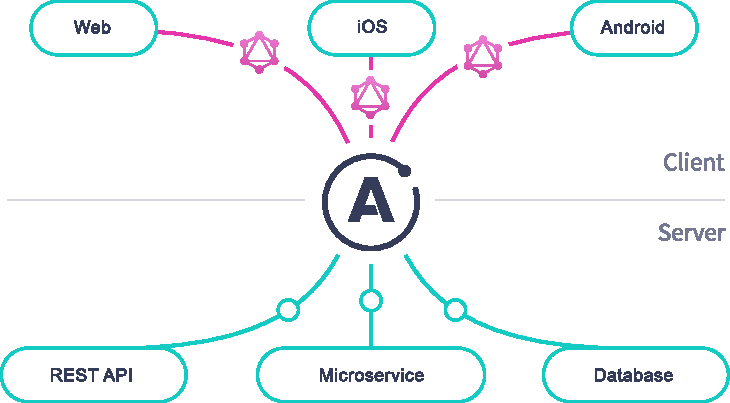
\includegraphics[scale=0.8]{obrazky-figures/apollo_server_diagram}
	\caption{Diagram architektúry Apollo Server. \cite{Apollo}}
\end{figure}

\noindent Apollo Server dokáže pôsobiť ako \emph{jednotná brána} pre všetky klientské aplikácie. Brána má predom definovanú schému, tzn. že klient presne vie aké operácie môže vykonávať a aké dáta môže očakávať späť.

% Slack API
\section{Slack API}
\label{theory:slack_api}
Aplikácia pre tímovú a pracovnú komunikáciu Slack umožňuje vývojárom vytvoriť vlastné aplikácie a prepojiť ich so Slackom pomocou ich \emph{otvorenej API}. \cite{SlackAPI} \\

\noindent Aplikácie môžu vykonávať niektoré akcie bežných užívateľov:

\begin{itemize}
	\item \emph{Odosielať správy} do rôznych koverzácií. \cite{SlackAPI}
	\item \emph{Čítať správy a konverzácie}. \cite{SlackAPI}
	\item \emph{Vytvoriť, archivovať a spravovať konverzácie}. \cite{SlackAPI}
	\item \emph{Reagovať na označenia} od užívateľov. \cite{SlackAPI}
\end{itemize}

\ldots no API aplikáciam umožňuje aj akcie mimo uživateľských práv:

\begin{itemize}
	\item \emph{Otvoriť dialógové okná} pre získanie alebo zobrazenie extra informácií. \cite{SlackAPI}
	\item \emph{Zostaviť interaktívne komponenty} na ktoré môzu reagovať \cite{SlackAPI}
	\item \emph{Vytvoriť a aktualizovať \uv{Home tab} (domovskú obrazovku)} kde môže užívateľ interagovať s~aplikáciou. \cite{SlackAPI}
	\item \emph{Definovať skratky} vďaka ktorým užívateľ môže rýchlo vykonať akcie v~aplikácií. \cite{SlackAPI}
\end{itemize}

\subsection{Block Kit}
Framework pre tvorbu uživateľského rozhrania pre Slack aplikácie, ktorý ponúka kompromis kontroly a flexibility pri budovaní rozhraní v~správach. \cite{SlackAPI}  Uživateľské rozhranie sa skladá pomocou blokov, ktoré sú vo forme JSON objekov prenášané do Slack aplikácie. Bloky sa delia na dve hlavné kategórie -- \emph{interactive} a \emph{layout} bloky. \\

\begin{lstlisting}[caption=Príklad jednoduchého bloku v~Slack aplikácií.]
	{
		"type": "section",
		"text": {
			"type": "mrkdwn",
			"text": "Hello, *World*!"
		}
	},
\end{lstlisting}

\bigskip

\noindent Bloky sa vkladajú do lineárneho zoznamu nazvanom \emph{view}, ktorý je následne odoslaný na príslušnú časť API, aby bol spracovaný. Niektoré bloky podporujú formátovanie pomocou modifikovanej verzie jazyka \emph{markdown}.

% Headless CMS
%---------------------------------------------------------------------------
\chapter{Headless CMS}
\label{theory:headless}
Headless CMS štandardne disponujú rozhraním REST\footnote{REST -- Representational State Transfer} alebo GraphQL, ktoré implementuje aj táto práca. Headless redakčný systém \emph{nerieši zobrazenie samotného obsahu}. Jediný spôsob ako obsah získať je využiť niektoré z~dostupných rozhraní poskytované konkrétnym riešením. Výhodou oproti tradičným redakčným systémom je možnosť získané dáta optimálne zobraziť na rôznych zariadeniach. 

\begin{figure}[h]
	\centering
	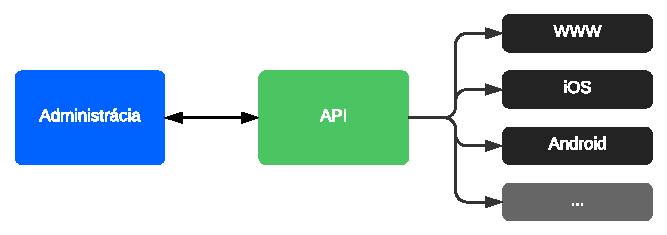
\includegraphics{obrazky-figures/headless_cms_graph.pdf}
	\caption{Ilustračná schéma generického headless redakčného systému.}
\end{figure}

\noindent Členenie obsahu v~takýchto redakčných systémoch je typicky v~dvoch vrstvách -- \emph{kategórie} a \emph{obsahové typy} (komponenty). \\

\noindent \emph{Kategórie} sú zoznamy združujúce jednotlivé komponenty, môžu byť homogénne (všetky prvky zoznamu sú jedného typu) alebo heterogénne (prvky zoznamu sú typicky iných typov). \\

\noindent \emph{Komponenty} sú atomickými prvkami headless redakčných systémov. Môžu nadobúdať rôznych typov, ktoré určujú ich vnútornú dátovú štruktúru. Typický príklad často používaných typov komponent je napríklad \texttt{prostý text} alebo \texttt{odkaz}. Niektoré headless redakčné systémy umožňujú vytvárať aj vlastné typy komponentov a tak si prospôsobiť dáta vlastným špecifickým potrebám.

% Strapi
\section{Strapi}
Najpopulárnejší Headless redakčný systém. Disponuje administračným panelom zostaveným na mieru, REST aj GraphQL rozhraním, systémom uživateľských práv a mnohými inými vlastnosťami. Tento redakčný systém má aj obchod s~aplikáciami, ktoré si môžu používatelia pridať a tým rozšíriť funkcionalitu. 

\blockquote[Dokumentácia Strapi.io \cite{StrapiDocs}]{Strapi je flexibilný, open-source\footnote{open-source -- otvorený kód, zväčša vyvíjaný komunitou} Headless CMS\footnote{CMS -- ang. content management system (redakčný systém)}, ktorý dáva vývojárom slobodu voľby ich obľúbených nástrojov a zároveň dovoľuje editorom jednoducho spravovať a distribuovať ich obsah.}

\noindent V~prípade, že by užívateľ Strapi mal nakonfigurovanú kolekciu s~názvom \uv{restaurants}, získanie počtu týchto kolekcií by mohlo vyzerať takto: \\

\begin{lstlisting}[caption=Príklad HTTP požiadavku na REST rozhranie Strapi.]
	GET "http://localhost:1337/restaurants/count" // Odpoved: 1
\end{lstlisting}

\bigskip

\noindent Pre použitie Strapi je nutné systém spustiť na vlastnej infraštruktúre, pripojiť k~predom vytvorenej relačnej databáze a celý systém nakonfigurovať.

% Netlify CMS
\section{Netlify CMS}
Netlify na rozdiel od väčšiny headless redakčných systémov nevyužíva pre ukladanie svojich dát relačnú databázu. Pre uloženie celého obsahu webovej aplikácie využíva repozitáre vytvorené v~prostredí \texttt{git}.

\blockquote[Dokumentácia Netlify CMS \cite{NetlifyDocs}]{Jadro Netlify CMS tvorí React [\ref{theory:react}] aplikácia ktorá využíva rozhranie pre prácu s~GitHub\footnote{\href{https://developer.github.com/v3/}{https://developer.github.com/v3/}}, GitLab\footnote{\href{https://docs.gitlab.com/ee/api/}{https://docs.gitlab.com/ee/api/}} alebo Bitbucket\footnote{\href{https://confluence.atlassian.com/bitbucket/}{https://confluence.atlassian.com/bitbucket/}} API.}

\noindent Netlify sa využíva väčšinou pre menšie stránky ako sú napríklad dokumentácie alebo produktové stránky, pretože umožňuje udržovať obsah relevantný k~danej verzií produktu.

% Návrh riešenia
%---------------------------------------------------------------------------
\chapter{Návrh riešenia}
Kapitola popisuje jednotlivé etapy vzniku návrhu služby, ktorá je predmetom tejto práce (ďalej ako \uv{\textbf{Slackify}}). Výsledný návrh vznikol po nadobudnutí požadovaných znalostí a analýz požiadavkov kladených na výsledný produkt.

Sekcia \ref{design:assignment} rozoberá zadanie práce, sekcia \ref{design:architecture} predstavuje architektúru systému aj s neúspešnými iteráciami, sekcia \ref{theory:data_types} popisuje špeciálne dátové typy navrhovaného systému. Posledná sekcia \ref{design:use_case} je venovaná konkrétnym prípadom užitia Slackify.

% Zadanie práce
\section{Zadanie práce}
\label{design:assignment}
Zadanie, ktorého celé znenie je priložené na \hyperlink{page.2}{strane 2}, popisuje výsledné riešenie práce ako \emph{headless} redakčný systém. Súhrn hlavných požiadaviek na systém je nasledovný:

\begin{itemize}
	\item Užívateľ systému by mal byť schopný spravovať obsah v~\emph{plnej miere} a bez obmedzení v~prostredí aplikácie Slack.
	\item Užívateľ by mal byť schopný začať využívať službu \emph{okamžite} po nainštalovaní do svojho pracovného prostredia v~aplikácií Slack. To znamená, že žiadna konfigurácia alebo nasadenie na vlastnú infraštruktúru by nemalo byť požadované.
	\item Všetky vytvorené dáta by mali byť dostupné cez verejné API.
	\item Systém by mal disponovať webovým rozhraním, odkiaľ by malo byť možné spravovať obsah a nastavenia.
\end{itemize}

\noindent Hlavnou výsadou práce nie je čo najväčšia flexibilita, ale jednoduchosť v~použití a možnosť rýchleho nasadenia. 

\subsection{Odchýlky návrhu od pôvodného zadania}
Slack API umožňuje vytvoriť uživateľské rozhranie zložené z~maximálneho počtu 100 blokov. Táto skutočnosť znamená, že nie je možné zobrazovať napríklad dlhé zoznamy prvkov. Pre tento dôvod je maximálny počet zobrazených prvkov v~zoznamoch Slack aplikácie limitovaný. Prvky zoznamov nad určený limit sú skryté a uzívateľ ich môže spravovať výhradne vo webovom prostredí. 

% Návrh architektúry
\section{Návrh architektúry}
\label{design:architecture}
Na začiatkoch navrhovania architektúry bola služba rozdelená do dvoch hlavných častí podľa vzoru \emph{backend} a \emph{frontend}. Frontend bola webová služba a backend poskytovala GraphQL bránu pre prístup k~dátam a logike pre frontend, ale slúžila aj ako prístupový bod pre koncových užívateľov headless redakčného systému a tiež ako bod pre komunikáciu so Slack API. Dáta boli ukladané v~relačnej databáze. \\

\noindent Aj keď v~prvopočiatkoch tvorby návrhu sa táto architekúra zdala ako vyhovujúca, neskôr sa ukázalo ako lepšia možnosť nasledujúce rozdelenie do štyroch menších služieb:

\begin{itemize}
	\item \texttt{frontend} -- Webová aplikácia poskytujúca prístup k~obsahu a nastaveniam headless redakčného systému. Táto časť zostala nezmenená.
	\item \texttt{service-slack} -- Serverová aplikácia zodpovedná za komunikáciu so Slack API. Udalosti a akcie prichádzajúce zo Slack aplikácie smerujú na túto službu, kde sú spracované a vyhodnotené.
	\item \texttt{service-private} -- Serverová GraphQL aplikácia poskytujúca logiku a prístup k~dátam \uv{frontend} službe.
	\item \texttt{service-public} -- Serverová GraphQL aplikácia poskytujúca prístup k~obsahu redakčného systému koncovým užívateľom.
	\item \texttt{database} -- Relačná databáza obsahujúca uživateľské dáta, nastavenia a obsah od koncových užívateľov.
\end{itemize}

\noindent Takáto architektúra sa oproti jednej veľkej backend službe ukázala ako výhodná z~dvoch hlavných dôvodov. Prvým dôvodom je \emph{omnoho jednoduchšia údržba} viacerých menších služieb (napríklad udržovanie logickej súborovej štruktúry bolo pri jednej monolitickej službe obtiažne). Druhým významným dôvodom je možnosť jednotlivé služby \emph{verziovať a vydávať samostatne}, pretože fungujú nezávisle jedna na druhej.


\begin{figure}[h]
	\centering
	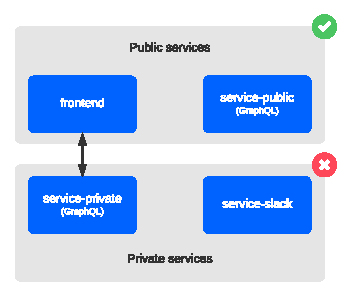
\includegraphics[scale=1.4]{obrazky-figures/architecture}
	\caption{Vizualizácia architektúry podľa návrhu.}
\end{figure}

Jednotlivé služby sú ešte rozdelené do dvoch skupín. \texttt{Frontend} a \texttt{service-public} sú služby dostupné pre verejnosť (\emph{public services}), \texttt{service-private} a \texttt{service-slack} sú pred verejnosťou skryté (\emph{private services}). 

% Dátové typy
\section{Dátové typy}
\label{theory:data_types}
Slackify je headless redakčný systém obsahujúci dva hlavné dátové typy -- \emph{collection} (kolekcia) a \emph{component} (komponenta). Pomocou týchto dvoch dátových typov je možné vytvoriť logickú štruktúru obsahu. U oboch dátových typov sa uchováva momentálny stav uverejnenosti \emph{published}, repretenzovaný dátovým typom boolean.

\subsection{Component}
Component (komponenta) je základná dátová struktúra v Slackify. Celý obsah redakčného systému je zložený komponent usporiadaných do kolekcií [\ref{design:collection}]. Každá komponenta má povinnú položku \emph{type} (typ), ktorá určuje ďaľšie zloženie štruktúry.

\subsubsection{Typ \uv{\texttt{Plain Text}}}
Najjednoduchší typ obsahujúci jediné povinné textové pole s názvom \emph{text}.

\subsubsection{Typ \uv{\texttt{Article}}}
Typ pre vytvorenie jednoduchého článku. Obsahuje povinné textové položky \emph{title} (titulok), \emph{content} (obsah článku) a nepovinnú textovú položku \emph{lead} (úvodný text).

\subsubsection{Typ \uv{\texttt{Link}}}
Typ pre vytvorenie hypertextového odkazu. Obsahuje povinnú textovú položku \emph{url} (cieľová adresa) a voliteľnú textovú položku \emph{text}.

\subsection{Collection}
\label{design:collection}
Collection (kolekcia) je zoznam slúžiaci pre kategorizovanie jednotlivých komponent. Každá kolekcia ich môže obsahovať 0 až $n$. Jedná sa o \emph{homogénny zoznam}, tzn. že pri tvorbe kolekcie sa vždy musí zvoliť práve jeden typ komponent z ktorých sa môže zoznam skladať. Každá kolekcia má povinnú položku \emph{name} (názov) a nepovinnú \emph{description} (popis).

% Diagram prípadov použitia
\section{Diagram prípadov použitia}
\label{design:use_case}
Priložené diagramy prípadov použitia zobrazujú chovanie systému z~pohľadu registrovaných užívateľov a zariadenia, ktoré sa snaží získať obsah z headless CMS.

\subsection{Viewer}
Každému novému užívateľovi, ktorý prepojí svoj účet v aplikácií Slack so Slackify je automaticky priradená základná užívateľská rola \emph{Viewer}. \\

\noindent Užívateľ s rolou \emph{Viewer} môže vykonávať nasledujúce akcie:

\begin{itemize}
	\item \texttt{Získať detail kolekcie/komponenty} -- Zobrazenie všetkých informácií o kolekcií alebo alebo komponente. Dáta je možné iba čítať, nie modifikovať.
	\item \texttt{Získať list kolekcií/komponent} -- Zobrazenie zoznamu kolekcií alebo komponent. Komponenty je možné zobraziť všetky alebo podľa pridelených kolekcií. Dáta je možné iba čítať, nie modifikovať.
\end{itemize}

\begin{figure}[h]
	\centering
	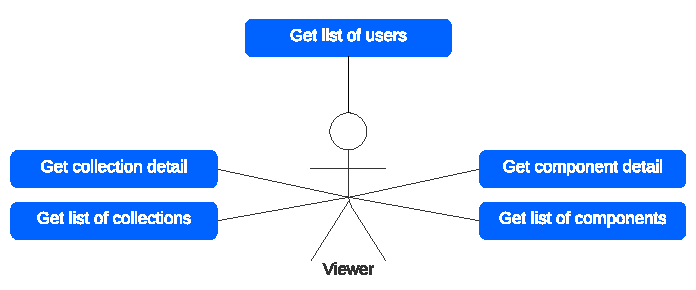
\includegraphics[scale=0.9]{obrazky-figures/viewer_use_case}
	\caption{Diagram prípadov použitia -- \emph{Viewer}.}
\end{figure}

\subsection{Author}
Užívateľská rola \emph{Author} zahŕňa všetky právomoci, ktoré mala rola \emph{Viewer} a rozširuje ich o možnosť vykonávať nasledujúce akcie:

\begin{itemize}
	\item \texttt{Vytvoriť kolekciu/komponentu} -- Po zadaní a potvrdení vstupných údajov je nová kolekcia alebo komponenta pridaná do databázy. Nové komponenty sú inicializované so stavom \emph{unpublished} (nepublikovaná).
	\item \texttt{Upraviť kolekciu/komponentu} -- Kolekcie alebo komponety je možné upraviť v~ľubovoľný čas. Jediná hodnota, ktorú nie je možné modifikovať je typ kolekcie alebo komponenty.
\end{itemize}

\begin{figure}[h]
	\centering
	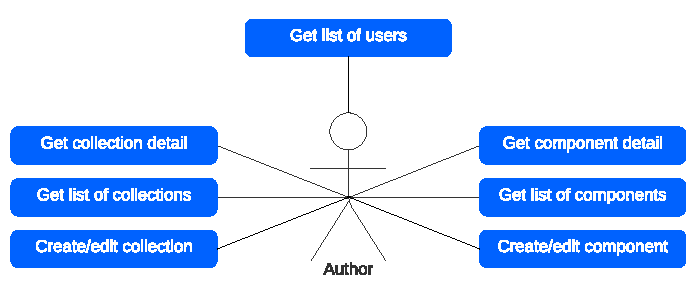
\includegraphics[scale=0.9]{obrazky-figures/author_use_case}
	\caption{Diagram prípadov použitia -- \emph{Autor}.}
\end{figure}

\subsection{Editor}
Užívateľská rola \emph{Editor} zahŕňa všetky právomoci, ktoré mala rola \emph{Author} a rozširuje ich o možnosť vykonávať nasledujúce akcie:

\begin{itemize}
	\item \texttt{Zmazať kolekciu/komponentu} -- Kolekcie alebo komponety je možné zmazať v~ľubovoľný čas. Pri zmazaní kolekcie sa zmazú aj všetky komponenty k~nej priradené.
	\item \texttt{Publikovať kolekciu/komponentu} -- Publikovaná kolekcia alebo komponenta je okamžite dostupná verejne. \emph{Editor} rovnako môže kolekcie alebo komponenty skryť.
\end{itemize}

\begin{figure}[h]
	\centering
	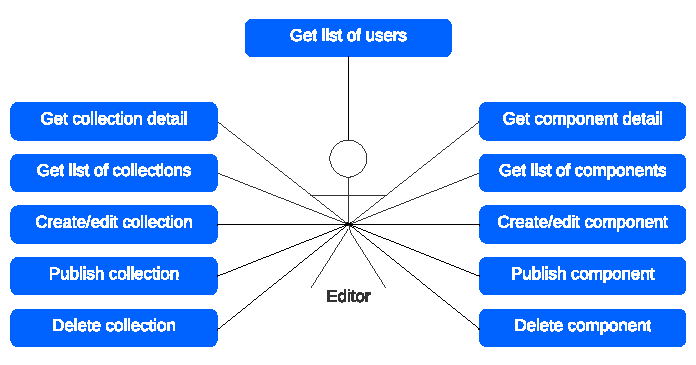
\includegraphics[scale=0.9]{obrazky-figures/editor_use_case}
	\caption{Diagram prípadov použitia -- \emph{Editor}.}
\end{figure}

\subsection{Owner}
Užívateľská rola \emph{Owner} je rola s najvyššími právomocami. Zahŕňa všetky právomoci, ktoré mala rola \emph{Editor} a rozširuje ich o možnosť vykonávať nasledujúce akcie:

\begin{itemize}
	\item \texttt{Zmeniť rolu užívateľa} -- Umožňuje modifikovať užívateľské role ostatných užívateľov. Užívateľ nemôže zmeniť rolu sám sebe. 
\end{itemize}

\begin{figure}[h]
	\centering
	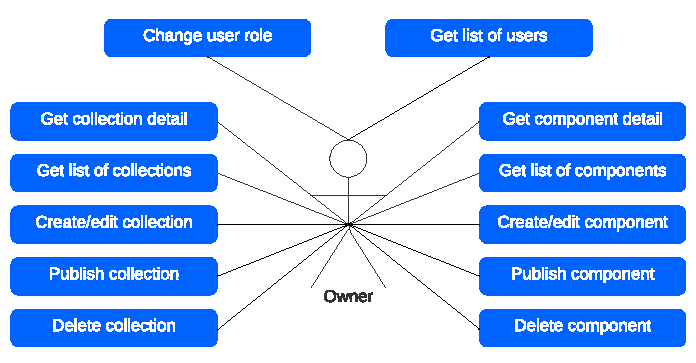
\includegraphics[scale=0.9]{obrazky-figures/owner_use_case}
	\caption{Diagram prípadov použitia -- \emph{Owner}.}
\end{figure}

\subsection{Zariadenie}
Obsah zo Slackify je možné získať z~verejného API (služba \texttt{service-public}) prostredníctvom akéhokoľvek zariadenia, ktoré dokáže komunikovať cez protokol HTTP. Pre ukážku diagramu prípadov použitia je na mobilnom telefóne nainštalovaná aplikácia, ktorá komunikuje s~rozhraním Slackify. \\

\noindent \emph{Zariadenie} môže v~prostredí Slackify vykonávať nasledujúce akcie:

\begin{itemize}
	\item \texttt{Vyžiadať detail kolekcie/komponenty} -- Informácie o jednej kolekcií alebo komponente je možné vyžiadať od API pomocou ich unikátneho ID.
	\item \texttt{Vyžiadať list kolekcií} -- Zariadenie si môže vyžiadať zoznam kolekcií. Zoznam kolekcií je v základnom nastavení zoradený chronologicky podľa času vytvorenia. Výsledky je možné zoradiť alebo filtrovať pomocou parametrov operácie.
	\item \texttt{Vyžiadať list komponent} -- Pomocou unikátneho ID kolekcie je možné vyžiadať k nej priradené komponenty. V prípade neuvedenia ID kolekcie je navrátený lisť všetkých komponent v danom Slack pracovnom prostredí (zoradené chronologicky podľa času vytvorenia). Výsledky je možné zoradiť alebo filtrovať pomocou parametrov operácie.
\end{itemize}

\begin{figure}[h]
	\centering
	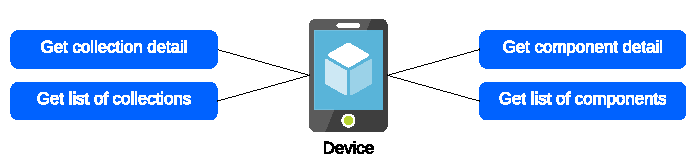
\includegraphics[scale=0.9]{obrazky-figures/device_use_case}
	\caption{Diagram prípadov použitia -- \emph{Zariadenie}.}
\end{figure}
